\documentclass[main.tex]{subfiles}
\begin{document}

\chapter{Benaderingen van verdelingen}
\label{cha:benad-van-verd}

\section{Limietstellingen}
\label{sec:limietstellingen}

\begin{st}
  De \term{centrale limietsstelling} (\term{CLT})\\
  Zij $X_{i}$ $n$ identiek verdeelde stochastische veranderlijken en $S = \sum_{i}X_{1}$.
  \[ \frac{S-n\mu}{\sqrt{n}\sigma} \rightarrow Z \]
  \[ \forall x \in \mathbb{R}:\ \lim_{n \rightarrow \infty} P\left(\frac{S - n\mu}{\sqrt{n}\sigma} \le x\right) = \Phi(x) \]
  \zb
\end{st}

\begin{st}
  De \term{stelling vna De Moivre-Laplace}\\
  Zij $X_{i}$ $n$ onafhankelijke stochastische veranderlijken die allemaal Bernoulli verdeeld zijn met parameter $p\in ]0,1[$ en $S = \sum_{i}X_{i}$.
  \[ \frac{S-n\mu}{\sqrt{n}\sigma} \rightarrow Z \]

  \begin{proof}
    Dit volgt meteen uit de centrale limietstelling.
    Immers $E[X_{1}] = p$ en $Var[X_{i}] = pq$.\needed
  \end{proof}
\end{st}

\begin{st}
  De \term{limietstelling van Poisson}\\
  Zij $X_{i}$ $n$ binomiaal verdeelde stochastische veranderlijken.
  Als $\lim_{n \rightarrow +\infty, p_{i} \rightarrow 0}np_{i} = \alpha$ geldt, dan ook:
  \[
  X_{i} \rightarrow X \text{ met } X \sim \mathcal{P}(\alpha)
  \]

  \begin{proof}
    Het volstaat te bewijzen dat de MGF van $\mathcal{B(n,p_{n})}$ naar die van $\mathcal{P}(\alpha)$ convergeert:
    \[ \forall t\in \mathbb{R}:\ \lim_{n\rightarrow +\infty}M_{\mathcal{B}(n,p_{n})}(t) = M_{\mathcal{P}(\alpha)}(t) \]
    \begin{align*}
       M_{\mathcal{B}(n,p_{n})}(t)
       &= (q_{n} + p_{n}e^{t})^{n}
       &= \left( 1 + \frac{(e^{t}-1)np_{n}}{n}\right)^{n}
       \overset{np_{n}\rightarrow \alpha}{\underset{n\rightarrow+\infty}{\longrightarrow}}
       e^{\alpha\left(e^{t}-1\right)}
       = M_{\mathcal{P}(\alpha}(t)
    \end{align*}
    We hebben hier gebruik gemaakt $\left(1 + \frac{a_{n}}{n}\right)^{n} \rightarrow e^{a}$ als $a_{n}\rightarrow a$.
  \end{proof}
\end{st}


\section{Practische benaderingen}
\label{sec:pract-benad}

\begin{de}
  Wanneer met een discrete verdeling $A$ benadert door een continue verdeling $B$ passen we de volgende \term{continu\"iteitcorrectie} toe:
  \[ P_{A}(X\le x) \approx P_{B}\left(X \le x+\frac{1}{2}\right)\]
  \[ P_{A}(X\ge x) \approx P_{B}\left(X \le x-\frac{1}{2}\right)\]
  \[ P_{A}(X=x) \approx P_{B}\left(x-\frac{1}{2} \le x \le x+\frac{1}{2}\right) \]
\end{de}

\begin{figure}[H]
  \caption{Benaderingen}
  \centering
    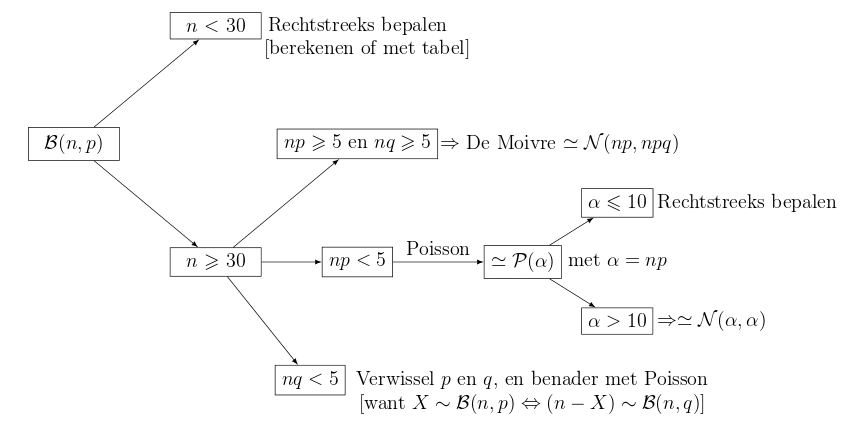
\includegraphics[width=\textwidth]{assets/benaderingen.png}
\end{figure}


\end{document}

%%% Local Variables:
%%% mode: latex
%%% TeX-master: t
%%% End:
